\documentclass[12pt,a4paper,leqno]{report}

\usepackage[T1]{fontenc}
\usepackage[english]{babel}
\usepackage{amsthm}
\usepackage{amsfonts}
\usepackage{amsmath}
\usepackage{amssymb}
\usepackage{graphicx}
\usepackage{hyperref}
\usepackage{tikz}

\usetikzlibrary{matrix}

\newcommand{\R}{\mathbb{R}} \newcommand{\C}{\mathbb{C}}
\newcommand{\Q}{\mathbb{Q}} \newcommand{\N}{\mathbb{N}}
\newcommand{\No}{\mathbb{N}_0} \newcommand{\Z}{\mathbb{Z}}
\newcommand{\diam}{\operatorname{diam}}

\theoremstyle{plain}
\newtheorem{equa}[equation]{Equation}
\newtheorem{lem}[equation]{Lemma}
\newtheorem{prop}[equation]{Proposition}
\newtheorem{cor}[equation]{Corollary}

\theoremstyle{definition}
\newtheorem{defi}[equation]{definition}
\newtheorem{conj}[equation]{Conjecture}
\newtheorem{example}[equation]{Example}

\theoremstyle{remark}
\newtheorem{note}[equation]{Note}

\pagestyle{plain}
\setcounter{page}{1}
\addtolength{\hoffset}{-1.15cm}
\addtolength{\textwidth}{2.3cm}
\addtolength{\voffset}{0.45cm}
\addtolength{\textheight}{-0.9cm}

\graphicspath{{../figures/}}

\title{Applying Bayesian Hierarchical Models to N-of-1 Trials}
\author{Tuomo Kareoja}
\date{\today}

\begin{document}

\maketitle

\tableofcontents

\chapter*{Introduction}\label{intro}
\addcontentsline{toc}{chapter}{Introduction}

In clinical practice, N-of-1 trials are multiple crossover trials conducted on a
single patient, where treatment periods are formed into multiple blocks each
containing at least one period of each treatment under
consideration\ \cite{nofone}. By comparing the measurements taken during different
treatment regimes over multiple blocks, the most suitable treatment option can
be chosen for the particular patient studied.

In the following pages, we will walk trough a concise explanation of the
experimental design of N-of-1 trials and how we can statistically model them,
given the kinds of challenges their design poses. We then follow up with how to
apply Bayesian inference with these models and estimate the effectiveness of different
treatments, highlighting how Bayesian methods can give needed flexibility when
running N-of-1 trials by not relying on hypothesis testing tied to a
prespecified study design. We then consider the case when there are multiple
similar N-of-1 trials and show how it is possible to pool the information from
these with hierarchical Bayesian methods, without loosing sight of the goal of
N-of-1 trials: to find the best treatment for each individual
patient. Finally, we end by with a complete example of analyzing multiple N-of-1
trials with hierarchical Bayesian methods with Python and PYMC3-package using
simulated data.

\chapter{What Are N-of-1 Trials?}\label{nof1}

In the assessment of any medical treatment the ``gold standard'' is a randomized
controlled trial (RCT), where subjects are randomized to two or more groups that
are given different treatments or no treatment at all. The measurements from
these groups are then compared and a result derived about which treatment is
most effective on average. This design takes into account unknown factors that
might make some patients more suspectable to certain treatments by forming the
groups randomly and thus, on average, distributing these patients evenly between
groups. By comparing the groups against each other and not just to the same
patients at the beginning and end of the study, it also takes into account time-related
effects like the natural progression of a disease. Despite its unquestionable value
in finding general effects, this method can run into problems when we
try to apply its results to individual patients in clinical practice.

Knowing the best treatment on average might not help much in finding the right
treatment for a particular patient if the variability in treatment effectiveness
between patients is high. Although we can use covariates like age, gender, or
a certain gene variant to explain the variance between patients in RCT:s, there
can still be lots of unexplained between-patient variance left. Some
of this variance is of course caused by random factors like measurement error,
but a significant part might be caused by real differences between the patients\ \cite{HTE1, HTE2, HTE3, HTE4}.
In other words, there might be individual factors that explain the variability
of the efficacy of different treatments between patients that might either be
too specific to be considered in an RCT study or unknown and thus impossible to
analyze in this kind of experimental design.

Another problem with RCTs is the peculiarity of their participants. It is
a common practice to accept patients to RCTs only if they don't suffer from any
medical issue besides the one that is being studied. This lack of comorbidity
makes it easier to get clear results by removing confounding factors, but at the
same time this lowers the external validity of the results, because in the real
world patients often suffer from multiple medical issues simultaneously. Because of this, it might be possible that even when the scientific
literature provides clear results about the relative effectiveness of different
treatments, these results don't generalize that well to the kinds of
patients the clinical practitioner sees daily in her office.\ \cite{HTE1}

N-of-1 trials can be used to patch the holes in the knowledge that RCTs cannot
fill by changing the focus of the study from group averages to the individual
patients. In N-of-1 studies, instead of comparing groups with different treatments,
the comparisons are made across time with a single patient using different
treatments. In this design multiple treatments are tried sequentially in periods
that are formed into blocks each of which contains a treatment period of each
treatment option under consideration at least once. Measurements are taken throughout the
study and, depending on the
ease of measuring the outcome of interest, these could be taken just
once per treatment period, or even multiple times per day. Each block includes a
period of each treatment under consideration in random or balanced order to take
into account time-related effects. A simple example would be an ABBA design that
includes two blocks within which the two treatments A and B are assigned in a
balanced order.

Depending on the treatments considered, there might also be a so-called
``washout'' period between treatments, where the patient does not receive any
treatment, and her state is allowed to return to baseline. This method is used to
prevent treatment interactions that could make it difficult to analyze the
results or could be dangerous to the patient. If the treatments being studied
allow it, N-of-1 trial can also use the double-blind method, where both the patient
and the person administering the treatment don't know which treatment is currently used, and placebo
treatment, where one of the treatments only resembles treatment, but does not
contain any active ingredient (pharmacological or otherwise).

Below is a schema of a more complex N-of-1 trial with three treatments A, B and C,
random assignment of treatments within blocks, three measurements within each
treatment period and washout periods between treatments:

\bigskip
{
    \centering
    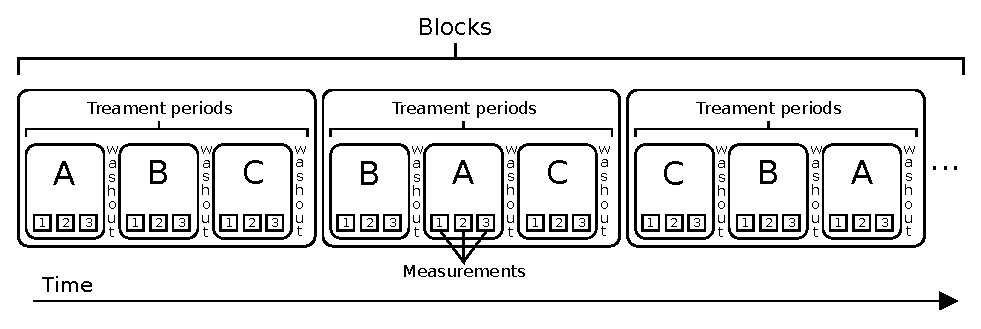
\includegraphics{n-of-1_schema.eps}
    \par
}
\bigskip

The stated aim of N-of-1 trials is quite different from RCT:s: where the latter
tries to generalize results to population and find which treatment is best in
general, the N-of-1 trial tries to only generalize to the patient in question.
This means that whereas comorbidity and other factors that cause systematic
variation between the patients in treatment outcomes are a problem in RCT:s,
these are not an issue in N-of-1 trials because there is no need to generalize
beyond the one patient. There is also often no actual need to know what is
causing a certain treatment to work better or worse, as long as it is not
because of measurement errors or time-related effects.

Use of N-of-1 trials is appropriate in situations where there are multiple
treatment options but there is no prior knowledge of which of these would be
best, when there is known to be considerable variability between patients in
treatment efficacy, or when there is reason to doubt that the results from
scientific literature generalize to the patient in question\ \cite{nofone}. This
would seem to make n-of-1 trials applicable to many situations, but there are
also multiple factors restricting their use\ \cite{nofone}.

Firstly, N-of-1 trials can only be used to study illnesses that are chronic,
progress slowly, and are at least somewhat stable. Also the treatment options
available must have noticeable treatment responses within a short timeframe.
Running the trials needs time to complete and fast-changing illness or slowly
effecting treatment make it either impossible to distinguish true effects from
the natural progression of the disease or make the length of the trials
impractically long. N-of-1 trials are also unsuitable for testing of
preventative treatments because the effects of these treatments are often
impossible to assess without comparisons to other patients who are not receiving
the treatment.

Secondly, running a N-of-1 trial is costly because of added expenses of training
the medical staff in the method, running the trial with all its measurements and
analyzing the data. This is means that it can be hard to find cases where using
this method is cost-effective and studies trying to make these kind calculations
have given mixed results\ \cite{costs}.

These limitations have kept the use of N-of-1 trials rare in clinical use, even
though they could potentially both increase the life quality of the patients and
lower the healthcare costs by finding the most suitable medications to patients that
might end up potentially using them for years. This state of affairs might be
changing fast though. Aging and environmental factors are changing the worlds'
disease burden so that a growing proportion of it is constituted by chronic
diseases\ \cite{diseaseburden}, of which common ones like non-acute cardiovascular
diseases and diabetes are excellent candidates for N-of-1 trials. Also the cost
of administering N-of-1 trials are dropping with the advent of cheap and reliable
health sensors like smartwatches and connected blood pressure monitors. For
example in diabetic patients it is now possible to get real-time readings of
blood insulin levels with minimal effort from the patient\ \cite{cgm}. These
factors mean that the popularity of this method could potentially rise
significantly in the future.

\chapter{Statistical Modeling of N-of-1 Trials}\label{modeling}

Even though the data created by the N-of-1 trials resembles traditional time
series data with autocorrelation between observations and repeated measurements
from the same study unit, there are additional complexities from the structure of repeating treatment periods. Trying to take into account all
the peculiarities of the study design could end up with model too complicated to
the small amount of data generated by a single study, so one must consider
carefully what factors actually \emph{need} to be incorporated into the model.

Simplest model that we could employ is to just count the number of blocks where
a treatment is considered ``better'' than others. The precise definition of
``better'' doesn't matter here. This way we arrive to a simple binomial model
where the number of ``successes'' \(X\) is the number of blocks where a
treatment is considered the ``best'' follows binomial distribution and the
probability of each treatment option of having \(k\) successes is given by:

\begin{def}\label{}
    \begin{equation}
        P(X = k) = {n\choose k}p^k{(1-p)}^{(n-k)},
    \end{equation}
\end{def}where \(k\) = number of blocks, where the treatments is considered the
``best'', \(n\) = total number of blocks and \(p\) = the probability of being
considered the ``best''.

This type of model is rudimentary at best because it fails to consider the
magnitude of the differences between treatment effects and does not take into
account the actual number of measurements within each treatment period. To take
these factors into account, more complex models are in order.

\section{Basic Models}\label{conti}

Before going further we make the assumption that the measurements are continuous
as this is probably the most common use case. Lets first look at a model where
we assume that there are no time-trends and no autocorrelation between
measurements. Let \(y_{mbpt}\) represent the outcome measured while on treatment
\(m\) within treatment block \(b\) within treatment period \(p\) at time \(t\).
The treatment periods are indexed within each block and time is indexed within
each treatment period:

\begin{def}\label{}
    \begin{equation}\label{allerrors}
        y_{mbpt} = \mu_m + \gamma_b + \delta_{p(b)} + \epsilon_{t(p(b))},
    \end{equation}
\end{def}where \(\gamma_b \sim N(0,\sigma^2_{\gamma})\), \(\delta_{p(b)} \sim
N(0,\sigma^2_{\delta})\), and \(\epsilon_{t(p(b))} \sim
N(0,\sigma^2_{\epsilon})\)

This model assumes all treatment effects \(\mu_m\) to be constant. Within the
normally distributed terms \(\gamma_b\) represents random block effects,
\(\delta_{p(b)}\) random period effects and \(\epsilon_{t(p(b))}\) random within
period errors. We could choose one of the blocks as a reference and set
\(\gamma_1 = 0\) and assume that within each block the between period effects
follow the same pattern, e.g.\ the difference between treatment period one and
two is the same within each block.

The random effects between blocks and treatment periods could represent for
example the random variations in the motivation of the patient and possible
changes in treating personnel within each block and treatment period. The random
within period errors represents the measurement error of single measurements
within treatment periods. The relative size of these terms is important
for effective design of the trial, because they determine if it is more be
beneficial for the statistical power of the study to add more measurements,
treatment periods or blocks.

If the measurements within blocks and within periods do not correlate, the
model\ \ref{allerrors} can be simplified by dropping \(\gamma_b\) and
\(\delta_{p(b)}\):

\begin{def}\label{}
    \begin{equation}\label{oneerror}
        y_{mbpt} = \mu_m + \epsilon_{t(p(b))},
    \end{equation}
\end{def}where \(\epsilon_{t(p(b))} \sim N(0,\sigma^2_{\epsilon})\).

This simple model is a natural fit in scenarios where there is just one
measurement within each treatment period.

\section{Incorporating time-trends into the model}\label{timetrends}

As the symptoms of the patient might not be completely stable (e.g.\ because
symptoms get worse with the progression of the disease) fitting some kind of
time-trend to the model is usually advisable. We can modify the model\ \ref{oneerror} from previous chapter to include a linear time-trend by adding an
intercept and slope of the time-trend. In this case the model can expressed more
concisely just in terms of the measurement \(y_t\) taken at time \(t\), where
time is indexed from the start of the study:

\begin{def}\label{}
    \begin{equation}\label{simpletimetrend}
        y_t = \beta_0 + \beta_1 t + \mu_t + \epsilon_t,
    \end{equation}
\end{def}where \(\epsilon_t \sim N(0,\sigma^2)\).

Here \(\beta_0\) is the intercept, \(\beta_1\) the slope of the time trend,
\(\mu_t\) the effect of the treatment given during time \(t\) and \(\epsilon_t\)
is the residual error at time \(t\). More complex time-trends can be introduced
by modifying the slope, for example by adding the term \(\beta_2 t^2\) to
introduce a quadratic trend.

Another effect dependent on time to take into consideration are period effects.
There might be some part of the trial that falls within a period that we presume
to have its own effect. An example of this kind of effect is if we study asthma
medications and part of the trial falls within the pollen season. A simple way
to model this is to use a dummy variable that takes the value 1 within the
period and 0 outside it. Extending the model\ \ref{simpletimetrend} with a period of constant
effect \(\beta_2\) we end up with:

\begin{def}\label{}
    \begin{equation}\label{}
        y_t = \beta_0 + \beta_1 t + \beta_{2}Z_t + \mu_t + \epsilon_t,
    \end{equation}
\end{def}where \(\epsilon_t \sim N(0,\sigma^2)\) and dummy variable \(Z_t = 1\)
when \(t \in (t_{period\,start} \ldots t_{period\,end}) \) and \(0\) otherwise.

Lastly, to take into account that treatment effects themselves can vary with
time, for example because treatment works better during periods of greater
disease severity, we can add a time-by-treatment interaction effect into the
model. For example in the case where we expect that the illness gets steadily
(linearly) worse with time, but the treatments compensate this by being
similarly more effective, we can extend the simple linear time-trend model\ \ref{simpletimetrend} by adding a second time related treatment term \(\gamma_t t\):

\begin{def}\label{}
    \begin{equation}\label{}
        y_t = \beta_0 + \beta_1 t + \mu_t + \gamma_t t + \epsilon_t,
    \end{equation}
\end{def}where \(\epsilon_t \sim N(0,\sigma^2)\)

\section{The Problem of Autocorrelation}\label{autocor}

A common occurrence in time-series data is the autocorrelation between
measurements so that there is some similarity between observations defined by a
function of the time lag between them. Often a good first response to this problem
is to add a time-trend to the model like we did previously. This
often removes a substantial proportion of the autocorrelation that could be
caused for example by the natural progression of the disease or seasonal variations
in its symptoms\ \cite{stat}. Unfortunately, in N-of-1 trials the carryover effects
from previous treatments and slow onset of treatment effects can lead to very
complex autocorrelation patterns that are hard to remove with just a simple time-trend.

Carryover effects refer to the lingering effects of the treatment even after it
has been stopped. This can make the treatment effects in the next treatment period
with a different treatment seem larger than they actually are or smaller in the
unfortunate and hopefully rare case where the previous treatment was actually
harmful. Carryover effects also encompass the effects of interactions between
sequential treatments, which could even be dangerous depending on the nature of
the treatments. On the other hand treatment effects that manifest slowly can
often give the opposite effect of carryover effects by making the treatments
look less effective than they really are during the first measurements of each
treatment period.\cite{stat}

To deal with these more devious sources of autocorrelation in our model we can
take two routes: moving average models and autoregressive models. In moving
average models the error is represented as depending on the previous error(s), by
expressing the measurement at time \(t\) as function of one or more previous
errors:

\begin{def}\label{}
    \begin{equation}\label{movingaverage}
        y_t = \mu_t + \epsilon_t + \rho\epsilon_{(t - 1)},
    \end{equation}
\end{def}where \(\mu_t\) is the effect of the treatment given at time t, \(\rho
\) is the correlation between consecutive errors and all errors \(\epsilon \sim
N(0,\sigma^2) \). Instead of making the measurement dependent on just the previous error the model
can be adjusted to include more a complex lag by adding more error terms with
bigger lag and including more \(\rho \) terms to denote the correlations between
them (\(\rho_1\epsilon_{t-1} + \ldots + \rho_x\epsilon_{t-x}\)).

In autoregressive models approach we express the autocorrelation in the
measurements themselves so that the measurement at time \(t\) is a function of
the measurement at \(t-1\):

\begin{def}\label{}
    \begin{equation}\label{}
        y_t = \rho y_{t-1} + \mu_t + \epsilon_t,
    \end{equation}
\end{def}where \(\mu_t\) is the effect of the treatment given at time \(t\),
\(\rho \) is the correlation between consecutive measurements and \(\epsilon_t
\sim N(0,\sigma^2)\) is the error term. Like with moving average model we could
also include more than just one lag by adding more lagged terms and correlation
terms.

Although it can make more intuitive sense to make the whole observation
dependent on the previous observation, it is important to recognize that in this
case the treatment effects \(\mu_t\) must be interpreted differently as they are
in this case conditioned on previous measurements.

Moving average models and autoregressive models are often combined by using both
methods of taking the autocorrelation into account simultaneously (ARMA-models), but as
amount of data produced in N-of-1 studies if often so small, taking this approach might not be advisable as it might make the model unnecessarily
complex.

Although we can try to solve problems created by the carryover effect and the slow
manifestation of treatment effect with modeling, a better way could be to take
measures to mitigate the effects in the study design itself. By having a long
enough washout period between different treatments, we can minimize the
carryover effect. If there are no harmful interactions between the treatment the
next treatment can be started within the washout period so that we minimize the
problem of slow treatment effects. If there are interactions to be taken into
consideration, the first few measurements at the beginning of each treatment
period could also just be dropped. By doing this we are of course throwing away
data, but we must be remember that if the measurements at the beginning of the
treatment period are mangled, this will also mangle our parameter estimates.
Trying to take these effects into account in our model will probably not
eliminate these effects completely and will increase the complexity of our
model.

\section{Non-continuous Measurements}\label{noncontinuous}

Up to this point we have assumed that the measurement used are continuous, but
we could of course have measurements that are binary, counts of events or
categorical. With these kinds of measurement the models need to reformatted so that
they don't presume normal distributions. Despite this the models still don't
have to differ much from the models presented above and the principals covered
before can be applied.

To modify previously presented models to work when measurements are not
continuous, we need to formulate them as generalized linear models. We do
this by keeping the right-hand sides in the same form but expressing the
left-hand side in terms of a link function of the mean of the probability
distribution of the outcomes. So instead of expressing the model in terms of
individual observations \(y_t\), we express it as the expected value of these
measurements conditional on the data \(E(Y|D)\) that we feed to the link
function. The link function allows us to model measurements with arbitrary
distributions, as now the link function can linearly depend on the parameters of
the model, rather than needing the measurements themselves to do so. We need to
do this to prevent the models from giving impossible predictions, e.g.\ negative
counts or probabilities.

Lets work with an example of a binary outcome measurements. In this case the
measurements \(y\) at time \(t\) follow the Bernoulli distribution \(y_t \sim
Bernoulli(p)\) where the the expected value of the distribution is the
probability \(p\) of observing the event in measurement \(y_t\). In this case
the suitable link function is the logit function
\(logit(p)=\log_e(\frac{p}{1-p})\). With this information we can now formulate a
simple model with a linear time trend:

\begin{def}\label{}
    \begin{equation}
        \log_e(\frac{p_t}{1-p_t})=\beta_0 + \beta_1 t + \mu_t,
    \end{equation}
\end{def}where \(p_t\) is the the probability of observing the event at time
\(t\) and \(\log_e(\frac{p_t}{1-p_t})\) are the log-odds of this event,
\(\beta_0\) is the intercept, \(\beta_1\) the slope of the time trend and
\(\mu_t\) the effect of the treatment given during time \(t\).

By first exponentiating and then using simple algebraic manipulation we can
express the model in terms of the probability \(p_t\):

\begin{def}\label{}
    \begin{equation}\label{}
        \frac{p_t}{1-p_t}=e^{\beta_0 + \beta_1 t + \mu_t}
    \end{equation}
\end{def}

\begin{def}\label{}
    \begin{equation}\label{}
        p_t=\frac{e^{\beta_0 + \beta_1 t + \mu_t}}{e^{\beta_0 + \beta_1 t + \mu_t}+1}=\frac{1}{1+e^{-(\beta_0 + \beta_1 t + \mu_t)}}
    \end{equation}
\end{def}

We notice that there are no error terms in this model. This is because we are
not modeling individual observations, but the expected value of these values
(probability of observing the event under treatment used at time \(t\) in this
case). Even though there is random variations in the individual observations,
when we talk about their expected value, there is just a single value with no
random errors. Apart from this difference we can see that we find the same model
from the denominator that we used when modeling a continuous measurement with a
linear time-trend in model\ \ref{simpletimetrend}, but without the
aforementioned error term. This means that to build the models described before,
we would just insert the right side of the equations into the denominator, apart
from the error term.

With numbers of events as measurements, instead of expressing the model in terms
of time, we can express it in terms of periods \(p\) that are of equal length
and indexed from the beginning of the experiment. The number of events during
period \(p\) follows a Poisson distribution \(y_p \sim Poisson(\lambda)\) and
the expected value of the distribution is the rate \(\lambda_p \) of the events
during period \(p\). For link function we use the natural log that is we have
\(\log_e(\lambda_p)\) on the left side of the equation. Once again using the
same simple model with linear time trend we end up with a model:

\begin{def}\label{oneerror}
    \begin{equation}
        \log_e(\lambda_p)=\beta_0 + \beta_1 r + \mu_{p},
    \end{equation}
\end{def}where \(\lambda_p\) is the the rate of events between measurements
during period \(p\), \(\beta_0\) is the intercept, \(\beta_1\) the slope of the
time trend and \(\mu_p\) the effect of the treatment given during period \(p\).
By simply exponentiating both sides we can express the model in terms of rate of
events:

\begin{def}\label{oneerror}
    \begin{equation}
        \lambda_t=e^{\beta_0 + \beta_1 t + \mu_t},
    \end{equation}
\end{def}where we now have the familiar linear model formula in the exponent on
the right side of the equation.

The case of categorical measurements is more complex as there are multiple
possible link functions depending on which way we want to model the
measurements, so we don't go trough all of them here. The one that is probably
the most relevant is the case when categorical measurements are ordinal, that is
they have a natural ordering (like in a Likert-scale). In this case the we can
use the cumulative logit as the link function. So if we assume that our ordinal
measurement has \(J\) categorical choices ordered from 1 to \(J\), we can model
the cumulative probability of getting a response \(y\) at time \(t\) that is at
least as ``severe'', by putting this to the logit function and using the same
basic model as before:

\begin{def}\label{oneerror}
    \begin{equation}
        \log_e\bigg({\frac{P(y_i \leq j)}{1 - P(y_i \leq j)}}\bigg)=\beta_0 + \beta_1 t + \mu_t,
    \end{equation}
\end{def}where \(\beta_0\) is the intercept, \(\beta_1\) the slope of the time
trend and \(\mu_t\) the effect of the treatment given during time \(t\). By
exponentiating and algebraic manipulation we end up with similar model as with
binary outcomes where we once again find the familiar linear model formula in
the exponent:

\begin{def}\label{}
    \begin{equation}\label{ord_exponentiating}
        \frac{P(y_i \leq j)}{1 - P(y_i \leq j)}=e^{\beta_0 + \beta_1 t + \mu_t}
    \end{equation}
\end{def}

\begin{def}\label{}
    \begin{equation}\label{ord_algmanipulation}
        P(y_i \leq j)=\frac{e^{\beta_0 + \beta_1 t + \mu_t}}{e^{\beta_0 + \beta_1 t + \mu_t}+1}=\frac{1}{1+e^{-(\beta_0 + \beta_1 t + \mu_t)}}
    \end{equation}
\end{def}

\chapter{Bayesian Estimation}\label{bayes}

Now that we have some models defined, we need to move into the next part of the
analysis and give estimates to the parameters in these models. There
are two broad ways to approach this task by using two different definitions of
probability. The first is frequentist inference, where we consider the ``true''
parameters of our model fixed, but unknown, and randomness only applies to the
process of creating our data. The second way is Bayesian inference, where we
consider the data to be fixed and instead of thinking about the parameters as
fixed parts of nature, we conceptualize them as probability distributions that
express our internal uncertainty about their true values.

Although both of these inference methods work for all the models covered before,
there are several factors that favor the use of Bayesian inference in N-of-1
studies that are related to their design and use context. We will return to these
later when we have first gone trough the principles of Bayesian inference.

\section{Principles of Bayesian Inference}\label{whybayes}

Bayesian inference is based on the Bayes' Theorem that states the probability of
an event conditional on another event:

\begin{def}\label{}
    \begin{equation}\label{bayesrule}
        P(A|B) = \frac{P(B|A)P(A)}{P(B)},
    \end{equation}
\end{def}where \(A\) and \(B\) are events and \(P(B)\) \(\neq \) 0. \(P(A|B)\) is the conditional probability of event \(A\) happening given that
event \(B\) happened and is called the posterior. \(P(A)\) is our initial
probability estimate for the event \(A\) called the prior. The quotient
\(\frac{P(B|A)}{P(B)}\) represent how much information event \(B\) gives about
event \(A\) happening. If this number is greater than 1, then event \(B\)
happening makes event \(A\) more likely and if it less than 1 is is less likely.
If the quotient is 1, event \(B\) gives no information about the probability of
event \(A\). Breaking the quotient down further \(P(B|A)\), called the likelihood, is the reverse of the posterior and tells us how believable it is to
see the event \(B\) given that event \(A\) happened. Finally \(P(B)\) in the denominator is called marginal likelihood and tells us the probability of
observing event \(B\) with or without event \(A\).

Instead of events, in our case we want to formulate the theorem with parameters
\(\Theta \) and the data \(D\), so that we get can estimate the posterior
probability (or likelihood in case of continuous parameter values) of our
parameters having certain values:

\begin{def}\label{}
    \begin{equation}\label{bayeswithparams}
        P(\Theta|D) = \frac{P(D|\Theta)P(\Theta)}{P(D)},
    \end{equation}
\end{def}where \(P(D)\) \(\neq \) 0. We could make it more explicit what the marginal likelihood \(P(D)\) stands for
by writing it as \(\sum_\Theta P(D|\Theta)P(\Theta)\) in the case when the parameter
value takes discrete values and \(\int_\Theta P(D|\Theta)P(\Theta) d\Theta \),
if they are continuous. That is, the possibility of observing the data with all
different combinations of the possible values of the parameters, taking into
account our prior belief in the probability of these value combinations.

To tie this formula into the models we introduced previously we can demonstrate
how this applies to a simple model with only the treatment effects \(\mu \) of
the given treatment and a random error \(\epsilon \) at time \(t\):

\begin{def}\label{}
    \begin{equation}\label{}
        y_t = \mu_t + \epsilon_t,
    \end{equation}
\end{def}where \(\epsilon_{t} \sim N(0,\sigma^2)\). Time \(t\) is indexed from
the beginning of the study. In this case when we want to estimate the parameters of the effects of the
treatments \(\mu_t\). For simplicity lets assume that only one treatment was
given so \(\mu_t\) is constant. Let's refer to this treatment effect simply as
\(\mu \). According to our model single observations follow a normal
distribution defined by constant \(\mu \) and the error term \(\epsilon_t \). As
our model assumes that the observations \(y_t\) are independent (no
autocorrelation included in the model) individual observations are defined as
\(y_t \sim N(\mu,\sigma^2) \) and the likelihood term in the bayesian formula is
a simple product of the probability density functions of a normal distribution
with mean \(\mu \) and variance \(\sigma^2 \) that the observations are
independent:

\begin{def}\label{}
    \begin{equation}\label{}
        P(Y|\mu, \sigma)
        =
        \prod_{Y}
        \frac{1}
        {{\sqrt {2\pi \sigma^2} }}
        \exp{ \left \{ \frac{-(y_t-\mu)^2} {2\sigma^2} \right \} },
    \end{equation}
\end{def}where \(Y\) represents all the observations.

To avoid the complexity of dealing with multiple unknown variables we assume
that \(\sigma \) is known. We will later come back to the case of multiple
unknown variables. Now we have to define only one prior distribution as there is
just one unknown parameter. We choose a normal distribution for the prior of
\(\mu \) that is defined by mean \(\lambda_0 \) and variance \(\delta_0^2 \),
whose values we define ourself based on our previous knowledge and beliefs:

\begin{def}\label{}
    \begin{equation}\label{}
        P(\mu)
        =
        \frac{1}
        {{\sqrt {2\pi \delta_0^2} }}
        \exp{ \left \{\frac{-(\mu-\lambda_0)^2} {2\delta_0^2} \right \} }
    \end{equation}
\end{def}

We could of course choose whatever distribution best matches our previous
knowledge and uncertainty about the parameter, but using a normal distribution
for prior when the likelihood also follows a normal distribution, we get some
nice algebraic properties that we will soon see.

Now the only missing term from our bayesian equation is the marginal likelihood
\(P(Y) \). When we express the term more precisely as the probability of getting
the data we observed over possible values of our unknown parameter \(\int
P(Y|\mu)P(\mu) d\mu \), we can see that as we integrate over all the possible
values of \(\mu \), the term is not dependent on the specific values of \(\mu
\). This means that the marginal likelihood is just a constant and as such does
not affect the shape of the posterior distribution, So the shape of posterior
distribution is defined by just by the likelihood and the prior \(P(\mu|Y)
\propto P(Y|\mu, \sigma^2)P(\mu) \). With some arithmetic manipulation we can
see that the posterior probability is actually a normal distribution with mean
\(\lambda_1 = \delta_1^2 \left( \lambda_0 \delta_0^{-2} + \sum_{Y} y \sigma^{-2}
\right) \) and standard deviation \(\delta_1^2 =
\frac{1}{\delta_0^{-2}+n\delta^{-2}} \):

\begin{align}\label{normalposterior}
    P(\mu|Y) & \propto P(Y|\mu, \sigma)P(\mu)                                                                 \\
             & =
    \prod_{t=1}^{n}
    \frac{1}
    {{\sqrt {2\pi \sigma^2} }}
    \exp{ \left \{ \frac{-(y_t - \mu)^2} {2\sigma^2} \right \} }
    \frac{1}
    {{\sqrt {2\pi \delta_0^2} }}
    \exp{ \left \{ \frac{ -(\mu - \lambda_0)^2 } {2\delta_0^2} \right \} } \nonumber                          \\
             & =
    \frac{1}
    {
        (2\pi)^{\frac{n+1}{2}}
        \sqrt{ \delta_0^2 \sigma^{2n}}
    }
    \exp{
        \left \{
        \frac{- \mu^2 + 2 \mu \lambda_0 - \lambda_0^2}{2\delta_0^2}
        -
        \sum_{t=1}^{n}
        \frac{y_t^2 - 2 \mu y_t + \mu^2}{2\sigma^2}
        \right \}
    } \nonumber                                                                                               \\
             & \text{Dropping the constant terms} \nonumber                                                   \\
             & \propto
    \exp{
        \left \{
        \frac{
            -\mu^2 (\sigma^2 + t\delta_0^2)
            + 2 \mu (\lambda_0 \sigma^2 + \delta_0^2 y_1 + \cdots + \delta_0^2 y_n)
            - (\lambda_0^2 \sigma^2 + \delta_0^2 y_1^2 + \cdots + \delta_0^2 y_n^2)
        }
        {2\delta_0^2 \sigma^2}
        \right \}
    } \nonumber                                                                                               \\
             & \propto
    \exp{
        \left \{
        \frac{
            - \mu^2
            + 2 \mu \frac{\mu_0 \sigma^2 + \sum_{t=1}^{n} \delta_0^2 y_t}
            {\sigma^2 + n \delta_0^2}
            - \left(
            \frac{
                \lambda_0 \sigma^2 + \sum_{t=1}^{n} \delta_0^2 y_t
            }
            {\sigma^2 + n \delta_0^2}
            \right)^2
        }
        {
            2 \frac{\delta_0^2 \sigma^2}{\sigma^2 + n\delta_0^2}
        }
        \right \}
    }
    \times
    \exp{
        \left \{
        -\frac{
            \lambda_0 \sigma^2 + \sum_{t=1}^{n} \delta_0^2 y_t
        }
        {
            2 \delta_0^2 \sigma^2
        }
        \right \}
    } \nonumber                                                                                               \\
             & \propto
    \exp{
        \left \{
        -
        \frac{
            \left(
            \mu
            -
            \frac{
                \lambda_0 \sigma^2 + \sum_{t=1}^{n} \delta_0^2 y_t
            }
            {
                \sigma^2 + n \delta_0^2
            }
            \right)^2
        }
        {
            2 \frac{
                \delta_0^2 \sigma^2
            }
            {\sigma^2 + n \delta_0^2}
        }
        \right \}
    } \nonumber                                                                                               \\
             & =
    \exp{
        \left \{
        -
        \frac{
            \left(
            \mu
            -
            \frac{
                \lambda_0 \delta_0^{-2} + \sum_{t=1}^{n} y_t \sigma^2
            }
            {
                \delta_0^{-2} + n \sigma_0^{-2}
            }
            \right)^2
        }
        {
            2 \frac{1}
            {
                \sigma^{-2} + n \delta_0^{-2}
            }
        }
        \right \}
    } \nonumber                                                                                               \\
             & \text{Recognizing that we have the ''right'' part of normal distribution and adding} \nonumber \\
             & \text{the constant part back in} \nonumber                                                     \\
             & \propto
    \frac{1}
    {{\sqrt {2\pi \sigma^2} }}
    \exp{
        \left \{
        -
        \frac{
            \left( \mu - \lambda_1 \right)^2
        }
        {
            2 \delta_1
        }
        \right \}
    }, \text{ where } \nonumber                                                                               \\
             & \delta_1^2
    =
    \frac{1}{\delta_0^{-2}+n\delta^{-2}}
    \quad\text{and}\quad
    \lambda_1
    =
    \frac{
        \lambda_0 \delta_0^{-2} + \sum_{t=1}^{n} y_t \sigma^2
    }
    {
        \delta_0^{-2} + n \sigma_0^{-2}
    }
    =
    \delta_1^2
    \left(
    \lambda_0 \delta_0^{-2} + \sum_{t=1}^{n} y_t \sigma^{-2}
    \right) \nonumber
\end{align}

So we ended up with a posterior distribution that has the shape of a normal
distribution. The trick where we ignored the marginal likelihood can be used
anywhere, but the fact that we could arithmetically solve that the posterior
follows a well-defined distribution is not a general occurrence. Usually we need
to go beyond arithmetic methods and solve the problem algorithmically.

\subsection{Challenges of Bayesian Inference}\label{bayesproblems}

Although the Bayes formula is conceptually simple, but when actually utilizing
it we run into two big difficulties. First is the common case when the
probability distributions of the prior and/or the likelihood or their product
are not well-defined distributions with known properties. This can make the
integral in the marginal likelihood impossible to solve analytically like we did
above. Even with discrete distributions similar problems emerge if the number of
possible parameter value combinations is very large (this can happen easily when
there are multiple parameters) as this makes just calculating the posterior
probability for each individual value unfeasible. The second problem is how we
should define our priors. If we have prior knowledge, we need to be able to
formulate our beliefs in a precise mathematic form and when we do not have prior knowledge we still
need to define a prior, but in this case it has to be defined so that it has
minimal effects on the posterior distribution.

\subsubsection{Dealing with the Marginal Likelihood}\label{bayesproblems}

As mentioned before, the marginal likelihood can often be impossible or
unfeasible to calculate analytically even in the case parameters with discrete
values where we don't need to solve a complex integral. A common solution to this,
that has been historically the only option, is to rely on so-called ``conjugate
priors``. These are priors that follow distribution which multiplied by
suitable likelihood function produce a posterior distribution that has the same
form as the prior distribution. A good example of this is our example above (\ref{normalposterior}) using a normal
distribution for the prior when the likelihood is also normally distributed. If
the likelihood function belongs to the exponential family of distributions, there
exists at least one corresponding conjugate prior distribution (often also in
the exponential family). For likelihood functions outside the exponential family
there are some cases where a conjugate prior exists, but these are rare.

The conjugate function method makes the denominator analytically solvable, but it
is in practice very limiting. First, we need to restrict ourselves when
modeling to only use models that create a suitable likelihood function with an existing conjugate prior. Second, it limits our options in defining our prior
beliefs as we have to be able to express them with the conjugate function. To
have a more general solution we need to abandon the search for an analytical
solution and tackle the problem algorithmically. We start this by noticing that
as the marginal likelihood is calculated over all possible parameter values, it is
not dependent on particular values of the parameter and is thus constant across
them. Therefore we can drop it from the Bayes' formula (\ref{bayeswithparams}) and state that the posterior
distribution follows the shape of the distribution of likelihood times prior:

\begin{def}\label{bayespropto}
    \begin{equation}
        P(\Theta|D) \propto P(D|\Theta)P(\Theta)
    \end{equation}
\end{def}

Even though we can't calculate the exact posterior probability any set value of
values for our parameters because we don't know the correct denominator, we now
have distribution whose shape is identical to the posterior. If we could take
samples from this distribution we could approximate the posterior distribution
with the probability distribution of the values of the samples. The general
method to get this kind of sample is the following:

\begin{enumerate}
    \item Pick a set of values for our parameters as our starting position in
          the parameter space. The starting location has to be a plausible set
          of values. We can check this As we can know that
          \(P(D|\Theta)P(\Theta)\) has the same shape as our posterior and so if
          the value of this function is zero when we pluck our set of
          parameter values in it, these values are impossible and should not be
          use as a starting point.
    \item Pick a second set of values for our parameters with some random method.
    \item Calculate the probability of moving from our current position in the
          parameter space to the second set of parameter values with the
          following formula:

          \begin{def}\label{randomwalk}
              \begin{equation}
                  p_{move\ to\ new\ location} = \min \bigg(\frac{P(D|\Theta = proposed\ set)P(\Theta = proposed\ set)}{P(D|\Theta = current\ set)P(\Theta = current\ set)}, 1 \bigg)
              \end{equation}
          \end{def}
          In other words, if the value calculated with the proposed parameter
          value set is higher than the value for the current set we always move
          to the new proposed location in the parameter space and if the value
          is lower we move there with a probability defined by the ratio of the
          two values.

    \item Generate a random number between 0 and 1 and move to the proposed
          location in the parameter space if the number is lower than the
          probability that we calculated in the previous step. Otherwise we stay
          in the same place.
    \item Mark down the values of our current location in the parameter space.
    \item Repeat from step 2.

\end{enumerate}

This method takes us on a random walk on the distribution with the steps defined
by the likelihood times prior, but as this is distribution has an identical shape
with the posterior function we indirectly end up with a representative sample of
values from the posterior distribution. So in actuality we have taken a random
walk in the posterior probability distribution, where we spend more steps in
parts of the distribution where the values are more likely. To end up with an
estimate of the posterior distribution we can now just divide the parameter
space into parts, calculate how many times we visited each of these parts and
divide this by the number of steps taken in total. We now have a proper probability
distribution that approximates the true posterior distribution. If we want a
more precise estimate, we can just take more steps and divide the parameter
space into smaller and smaller parts.

This algorithm is a general description of a group of algorithms called
Metropolis-Hastings algorithms. All of these methods follow the principles
above, but they differ in the way they decide where to move next. Although with
even very simple rules of picking a random proposed value the described will end
up exploring the whole posterior distribution eventually, more clever algorithms
can make this process much more efficient. By proposing steps that are more
likely in posterior distribution a clever algorithm can lower the chance of
proposing steps that have a high probability of being rejected and so assure
efficient moving trough the parameter space with less steps.

Metropolis-Hastings algorithms themselves are a part of a more broader group of
algorithms called Markov chain Monte Carlo methods that all are methods of
sampling from a probability distribution. The development of these methods has
been pushed forward by the need to have the sampling be as efficient as
possible, as even with the computational power of a modern computer, more complex
models can run into unfeasibly long computational times. On top of choosing the
right algorithm, there are lots of other things related to the computation to
consider when implementing Bayesian inference, but we will return to these later
with the example of practical implementation of this kind of calculation with
Python and PYMC3 package.

\subsubsection{How to Define the Priors?}\label{bayesproblems}

For the Bayesian formula to work we have to define a prior and this can be
trickier that it seems at first glance. Ideally the prior would codify our prior
beliefs and knowledge\ \cite{gelman, kruschke}, but trying to actually codify all we
know is a fool's errand, because of how complex this is and we are
anyway working with a model that is a simplified representation of reality. Even if
we aim for a more limited goal, codifying what we know (or think we know)
to mathematic formulas can be a tricky business. But it gets more
difficult when we consider that we are doing the study not just to convince ourselves
but also other people and we should try to capture the beliefs of our target audience.
Unless this target audience is easily available for questions and is highly mathematically minded,
this leads to multiple layers of uncertainty as we try guess what others
believe and then codify these beliefs with mathematical precision.

To avoid this hurdle the other option is to try to define some non-informative
priors that ``let the data speak for itself'', but this approach also has
problems. Firstly, defining priors that have no effects on the posterior can be mathematically
very difficult when we move beyond simple models\ \cite{gelman} and if we would need
to invest a lot of time finding these priors we should instead probably spend this time
to define proper informed priors. Second, non-informative priors do not always
seem so non-informative, when we actually know something about the issues.
Consider a case where are trying to predict if a patient has a rare disease
and we assign a uniform prior from 0 to 1 as this seems non-informative. This
prior will have the effect of moving the posteriors towards the
possibility of the patient actually having the disease. So if we definitely know
something about the phenomenon, a non-informative prior can work against these
beliefs.

Considered more broadly, chasing after truly non-informative prior is also
somewhat of a fool's errand if the data actually has ``something to say''.
If the data is informative, then lots of different priors that are somewhat weak
should lead to almost identical posterior distributions. On the other hand if the data is weak and we
have a weak prior, why are we even doing the analysis if we know that it will
give us almost no information?

As a compromise between having strong priors based on previous beliefs and knowledge and
letting the data stand on its own, Gelman et al.
suggest using weakly informative priors\ \cite{gelman}. These can be defined in two different
ways. First we can start with non-informative prior (when it is easily
available) and then add minimum information constraining the posterior results
to reality (e.g.\ object cannot move faster than light or the height of an adult human
must be between 50 and 300 cm). The other way is to start with strong informative
priors and then broaden these to take into account the uncertainty of
how applicable our priors knowledge is to the question at hand.

Because of how complex defining priors can get, this problem can act as an
additional limiter on how complex Bayesian models we can build. The more complex model, the more priors we
have to define and the more prior information and beliefs we could codify and
the more difficult this problem gets.

\section{Why Bayesian Inference Fits N-of-1 Studies}\label{whybayes}

As mentioned at the beginning of the previous chapter, both frequentist and
Bayesian inference can be used to estimate the parameter values of the models
described. The choice between these two methods is not just a technical one as both come
with different conceptions about the nature of probability and assumptions
related to this conception and these have serious implications on how we should
interpret the results and run the studies. Unfortunately for frequentist inference, its
assumptions fit the reality the N-of-1 trials poorly, and its estimates, and
especially their uncertainty, can be hard to communicate to a lay audience (doctors and patients).
Because of these issues, Bayesian inference can usually be recommended over
frequentist inference when analyzing and communicating the results of N-of-1
studies, even though it comes it with its' own complexities that we previously went over.

\subsection{Flexibility of Experimental Design}\label{whybayes}

The central tenet of frequentist inference is the assumption that same the
experiment could be in theory repeated with statistically independent results. Probability
is defined in relation to these hypothetical repetitions as a proportion of them
that would have some event of interest (e.g. over 5 tails with 10 coin tosses). To repeat the same experiment its design
needs to be defined precisely and this definition needs to be made before the
study has begun because the changes made to the design during the experiment
might be influenced by its results.

Lets take for example an experiment where we are trying to find out if a coin
is fair. For this purpose, we decide to flip the coin 20 times and count the number
of heads. Then we can model how ``typical'' the result we got would be for a fair coin. We do
this by calculating the distribution of heads from multiple 20 coin toss trials
assuming that the coin is fair. Then we can compare our actual result against this
distribution. If the result would be typical within this distribution, then we
can say that the null hypothesis stands and the coin is fair. The problem comes if we did
not actually decide to throw the coin 20 times beforehand, but first threw it 10 times, looked at
the results, though that we should get some more data, and then threw the rest 10. Now what
kind of distribution should we compare our results against? The length of the trials
seems to now hinge in some undefined way from the results of the first 10 coin tosses
that made us decide to keep tossing the coin some more.

This demand for predefined experiment designs can be especially problematic in N-of-1 studies
used in a clinical setting. There might be cases when some treatment seems
clearly better in the middle of an experiment and the patient (or the clinician)
wants to stop the experiment. As the subjects are real people, it would be
unethical to force them to continue the study just for the sake of statistical
rigor. There might also be a situation where a couple of treatments seem
promising, but the rest seem completely useless, and we would want to change the
design of the experiment on the fly to focus just on the promising treatments.
These changes to the predefined experimental design will brake frequentist
assumptions and make the inferences made with this method very difficult.

The possibility to stop the study or change the experimental design can be
incorporated to frequentist inference if we predefine the rules of when to
stop the experiment and under what circumstances the design should be altered
and how. Then we need to take these rules into account when performing the estimation
calculations which adds complexity is but is still possible. The problem is that it is questionable if we can actually
define and stick to these rules because of the human element: we would need to convince the patient that she should stop the experiment only in these predefined circumstances. This seems quite
unrealistic, as if there are any unforeseen problems with the treatments, it is
more than likely that the patient will want to stop whatever rules she sign to follow
beforehand.

With Bayesian inference doing on the fly modifications of the study design do not
cause such problems as with frequentist inference, as there is no assumption
about repeating the experiment. Instead of hypothesizing about future
experiment, we just take into account our prior information and the data created by
the current experiment. The changes to the experimental design modify what data
we get out of it, but don't brake any assumptions of Bayesian inference. This
adaptability is a big benefit when applying N-of-1 designs in a clinical setting, as
the unpredictable nature of the patients and treatment effects and all the other
practical considerations that could force changes to our experiment design don't
break the assumptions of the inference method.

\subsection{Richness and Communicability of the Estimates}\label{whybayes}

In N-of-1 studies, much consideration has to be given to the communication of the
results, both to the patient and the clinician administering the experiment. We
would like to portray not just the estimates of the effects of the treatments,
but also the uncertainty associated with these estimates. In frequentist
inference there are two options to communicate these facts. The first one is
maximum likelihood estimates combined with confidence intervals. Maximum
likelihood estimates are just point estimates of the most likely parameter values and don't
communicate any uncertainty. Confidence intervals of these parameter values communicate uncertainty, but
don't actually mark the most likely values of the estimate. A 95 \%
confidence interval, is often interpreted wrongly as including the true value of
the parameter with 95 \% change, but the real meaning is that if we repeated the
experiment indefinitely 95 \% of the 95 \% confidence intervals would include
the true parameter value. This is because in frequentist interpretation of
probability, true parameter values are not random but fixed, so a single
confidence interval either does or does not include the true value. This
confusing definition makes confidence intervals a poor choice of presenting the
uncertainty of the estimates to a lay audience as they might create lots of misinterpretations and
even when interpreted correctly are hard to grasp.

The second frequentist communication tool are p-values of hypothesis tests. We
might define a null hypothesis that the parameters of the effects of different
treatments are equal and calculate the likelihood to obtain the data or a more
extreme version of it if this is indeed the case. This would give us a more
easily communicable way to portray the probability to obtain the data if the null
hypothesis is true. If the p-value is low we could say with confidence
that there is real differences between the effectiveness of the treatments. The
problem is that this actually gives us very little useful information, as we
would also like to how big the differences in the treatments' effectiveness
could realistically be.

A Bayesian approach to inference gives us richer and more easily communicable
information about the estimates because it gives us a distribution as a
result in the form of the posterior distribution. With this is we can easily point out the plausible values
with the tops of this distribution and the uncertainty with how flat the
distribution is. The usual misinterpretation of the confidence intervals as
containing the true value of the parameter with a certain probability is actually
the right interpretation for Bayesian credible intervals, that contain certain
percentage of the probability mass of the posterior distribution and so have a
defined chance of containing the true value of the parameter. Bayesian method itself also seems to fit really well with the ways that clinicians conceptualize
their practice of arriving to  diagnosis for a patient as updating their beliefs
(i.e.\ priors) with the new information gained from new observation such as test
results\ \cite{clinbayes}.

\chapter{Combining Information From Several N-of-1 Trials With Hierarchical
  Models}\label{hierarchicalbayes}

Let's say we have our N-of-1 trial set up nicely and we have a good model for analyzing the
results. After running the first trials we continue to perform the same kind of setup
with multiple patients as the treatments we are considering seem to have lots of
individual variation in their effectiveness. Running these experiments separately is
fine, but one might wonder could these separate trials be somehow combined. Of course, we could pool the data and run a group-based
analysis about what treatments seems to be the best in general, but there is a better
way to keeps true to the goal of N-of-1 experiments of finding the best treatment for
each \emph{individual patient}.

In the Bayesian framework we can do this by using hierarchical
models where each model parameter is imagined to come from ``higher'' distributions
that is controlled by its own parameters. Where individual parameters represent the
individual patients the distribution where they come from represents the tendencies of
the population where the patients are drawn from. For example we could assume that the
effectiveness of a certain treatment to be normally distributed within a
population and the effectiveness of this treatment for a single patient
comes from this distribution and its shape tells that certain values for
patient-level parameters are more or less probable.

% TODO check where you have to put the exponent in the variance parameters

\bigskip

\begin{tikzpicture}

    \matrix[matrix of math nodes, column sep=10pt, row sep=40pt] (mat)
    {
        \ & \theta_{\mu}, \tau_{\mu}, \alpha_{\theta}, \alpha_{\beta} & \ \\
        \ & \mu, \sigma, \beta & \ \\
        \theta_1, \tau_1 & \ldots & \theta_p, \tau_p \\
        y_{1,1}, \ldots, y_{n, 1} & \ldots & y_{1, p}, \ldots, y_{n, p} \\
    };

    \draw[->,>=latex] (mat-1-2) -- (mat-2-2);

    \draw[->,>=latex] (mat-2-2) -- (mat-3-1);
    \draw[->,>=latex] (mat-2-2) -- (mat-3-3);

    \draw[->,>=latex] (mat-3-1) -- (mat-4-1);
    \draw[->,>=latex] (mat-3-3) -- (mat-4-3);

    \node[anchor=east] at ([xshift = -35pt]mat-1-1)
    {};

    \node[anchor=east] at ([xshift = -35pt]mat-2-2)
    {$\mu \sim \text{N}(\theta_{\mu}, \tau_{\mu}^2), \sigma \sim
    \text{HalfCauchy}(\alpha_{\sigma}), \beta \sim \text{HalfCauchy}(\alpha_{\beta})$};
   
    \node[anchor=east] at ([xshift = -35pt]mat-3-1)
    {$\theta_p \sim \text{N}(\mu, \sigma^2), \tau_p \sim \text{HalfCauchy}(\beta)$};

    \node[anchor=east] at ([xshift = -35pt]mat-4-1)
    {$y_{n,p} \sim \text{N}(\theta_p, \tau_p^2)$};

\end{tikzpicture}

\bigskip

The elegance of this method comes from the fact that, even though we now have a group
level parameter (the distribution of effectiveness of the drug in the population) we
still keep the individual patient level parameters and these can still be wary different
between the patients. The patient-level data is used to inform us about the population
level parameters and this in turn affects the patient level parameters. In principle we
are pooling the information from multiple patients and using this data adjust our
patient-level inference, but the pooling is done intelligently so that for example if
patients seem very different there is very little effect, but if the parameters from all
but one of the patients is clustered very close to each other, we adjust the parameter
estimates of this one patient closer to the other patients.

The question now becomes, how we apply the Bayesian formula in this case?

To start exploring this lets first look in more detail the case when we have
more than one parameter in our model. We alluded to this already previously
when we talked about multiple parameters, but we did not go into details
there about how this affects the formulas practically. Lets take an example where
we have two parameters instead of one, slot them into the familiar Bayes’ rule
and see how it applies to the joint parameter space:

TODO: explain the steps in more details

\begin{def}\label{conjugatebayesrule}
    \begin{equation}
        p(\theta, \sigma|D) \propto p(D|\theta, \sigma) p(\theta, \sigma) = p(D|\theta) p(\theta|\sigma) p(\sigma)
    \end{equation}
\end{def}

We start from the basic definition of the posterior and the apply the Bayes rule, but ignore
the denominator as we learned previously that if we just want to know the shape of the
posterior these has no effect on it can be dropped. Next we applied

We can see that the data \(D\) depends only on the value of parameter \(\theta \), so that
if the value of \(\theta \) is set, then the data are independent of all other
parameter values. Similarly, the value of \(\theta \) depends conditionally only
the value of \(\sigma \) and \(\sigma \) is an independent variable.

These kinds of dependencies among parameters are useful in several respects.
First, the dependencies are meaningful for the given application, e.g.\ we can
model that the treatment effect for a single patient as an instance from a
broader population distribution of this effectiveness. Second, because of the
dependencies across parameters, all the data can now jointly inform all the
parameter estimates. The reduction of variance in the estimators that this
effect causes, is generally referred by the term ``shrinkage''.

In general, shrinkage in hierarchical models causes lower-level parameters to
a shift toward the modes of the higher-level distribution. If the higher-level
distribution has multiple modes, then the low-level parameter values cluster
more tightly around those multiple modes, which might actually pull some
low-level parameter estimates apart instead of together. The greatest thing
is that if we don't explicitly set the parameter values of the higher-level
distributions, the amount of shrinkage is actually informed by the data so that
similar observed data points from lower-level distributions lead to ``tighter''
estimates for the higher-level distributions and in this in turn leads to
greater shrinkage.

\chapter{Example of a Hierarchical Bayesian Analysis Using Simulated
  Data}\label{example}

Imagined experimental design

\section{Simulating the Data}

\begin{def}\label{simulationmodel}
    \begin{equation}\label{}
        y_t = \mu_i + t\beta_i + Z_t\theta_i + \epsilon_t + \rho_i\epsilon_{t-1}
    \end{equation}
\end{def}where \(\mu_i\) is the baseline of the patient \(i\), \(\beta_i\) is
the trend, \(\theta_i\) is the treatment effect with \(Z_t\) being an indicator
variable that is 1 when \(t\) is within a period where treatment was applied and
0 otherwise. \(\epsilon_t \sim N(0,\sigma_i^2) \) is the error term at \(t\) and
\(\rho_i\) is the is the correlation between consecutive errors.

So we have a data generating model with both and trend and lag 1 autocorrelation
making the generated model more complex. The trend and autocorrelation are parts
of the generation process that likely cannot be modeled with the generated data
because of limited observations. This way the example tries to be more realistic
by having the data generation function to be such complexity that it cannot be
fully modeled and some decisions have to be made of how to try to approximate
the process with a simpler model.

These patient-level terms are generated from the population level distributions

\begin{def}\label{populationparameters}
    \begin{equation}
        \mu_i \sim \mathcal{N}(\mu,\sigma^2)
    \end{equation}
    \begin{equation}
        \theta_i \sim \mathcal{N}(\theta,\sigma^2)
    \end{equation}
    \begin{equation}
        \sigma_i \sim Beta(\alpha, \beta)
    \end{equation}
    \begin{equation}
        \rho_i \sim InvGamma(\alpha, \beta)
    \end{equation}
\end{def}

\bigskip
{
    \centering
    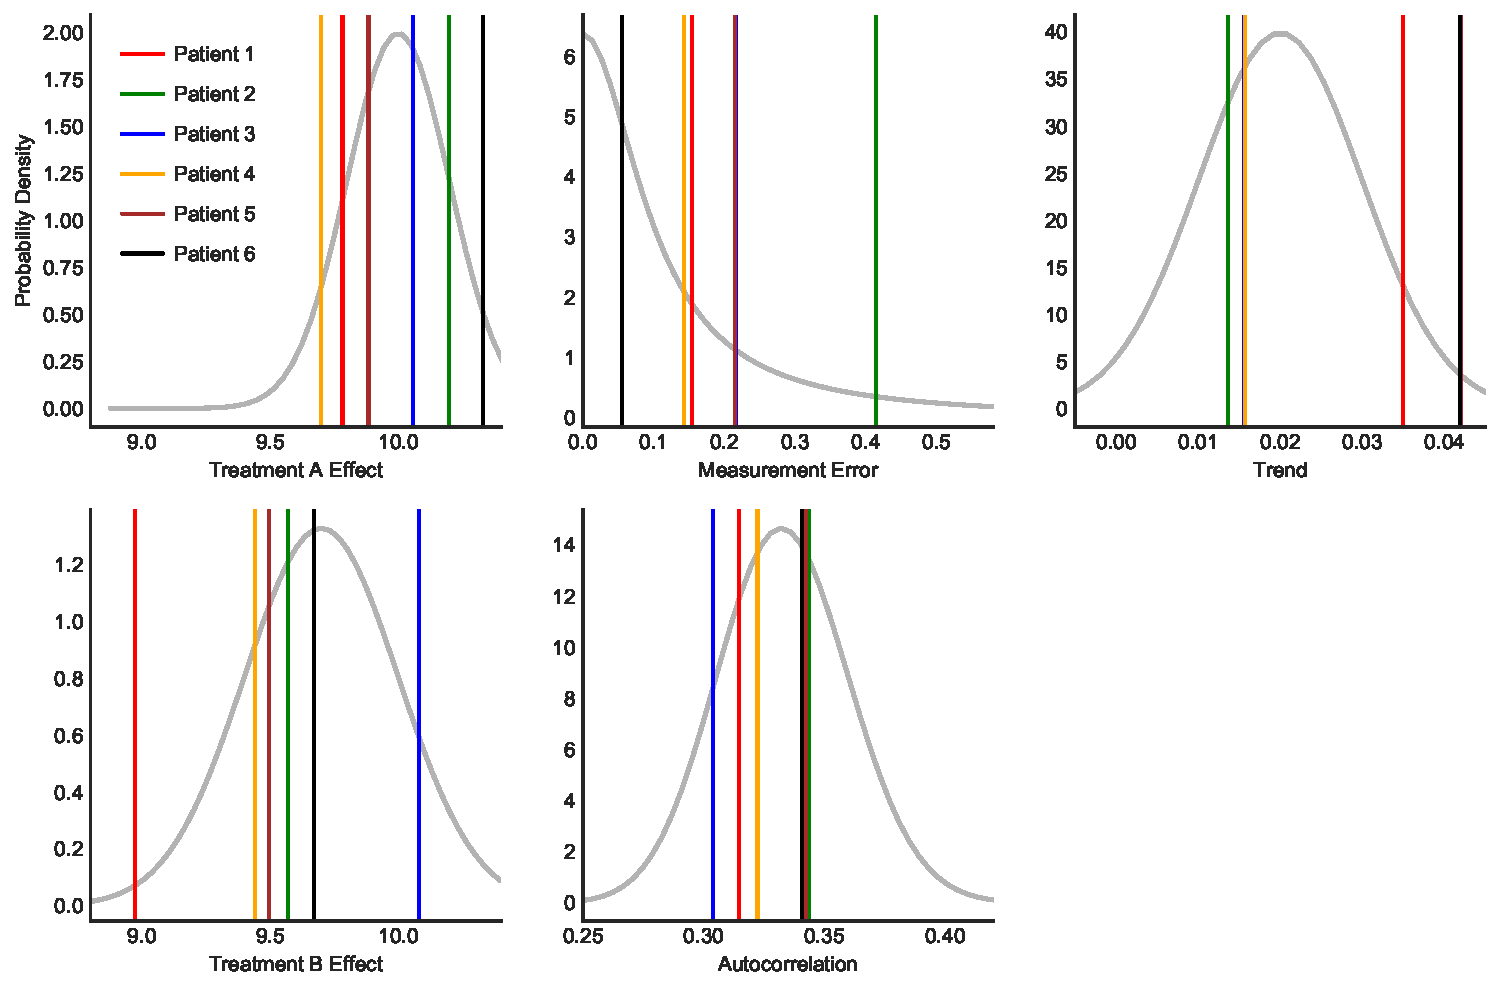
\includegraphics[width=\textwidth,height=\textheight,keepaspectratio]{population_parameter_distributions.pdf}
    \par
}
\bigskip

\bigskip
{
    \centering
    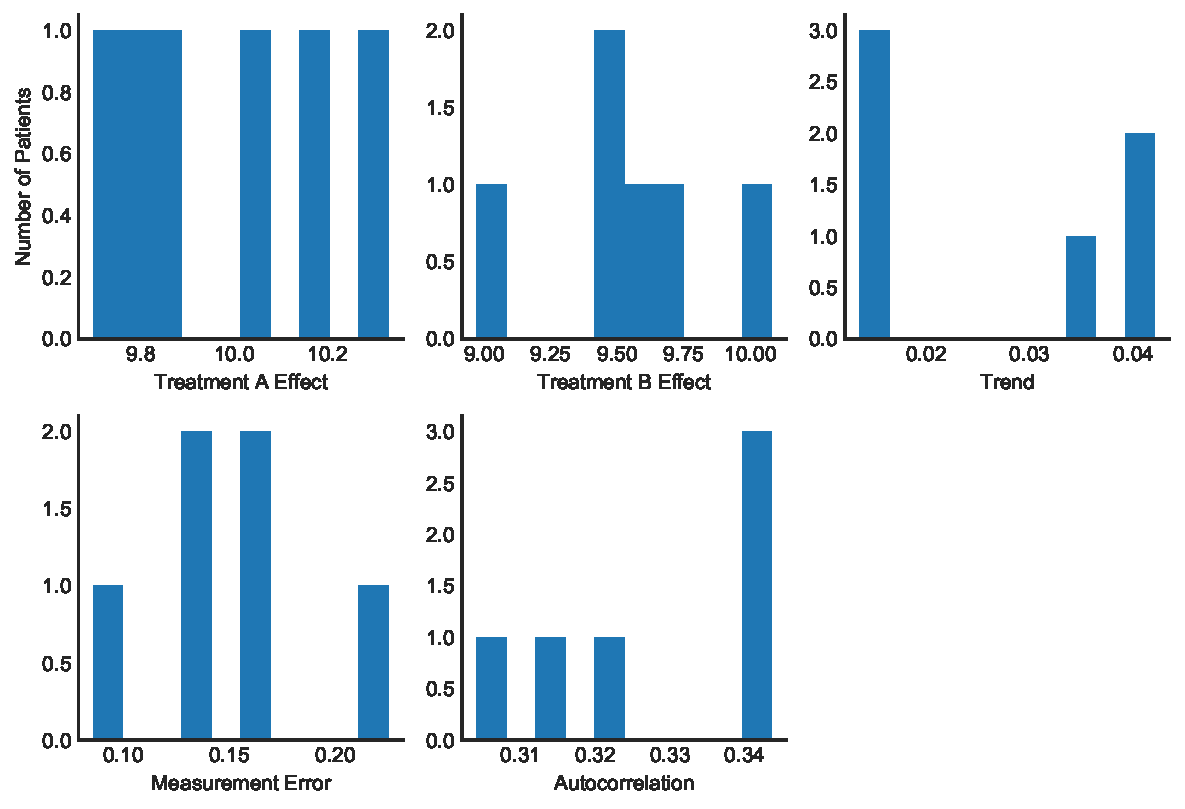
\includegraphics[width=\textwidth,height=\textheight,keepaspectratio]{patient_parameter_distribution.pdf}
    \par
}
\bigskip

\bigskip
{
    \centering
    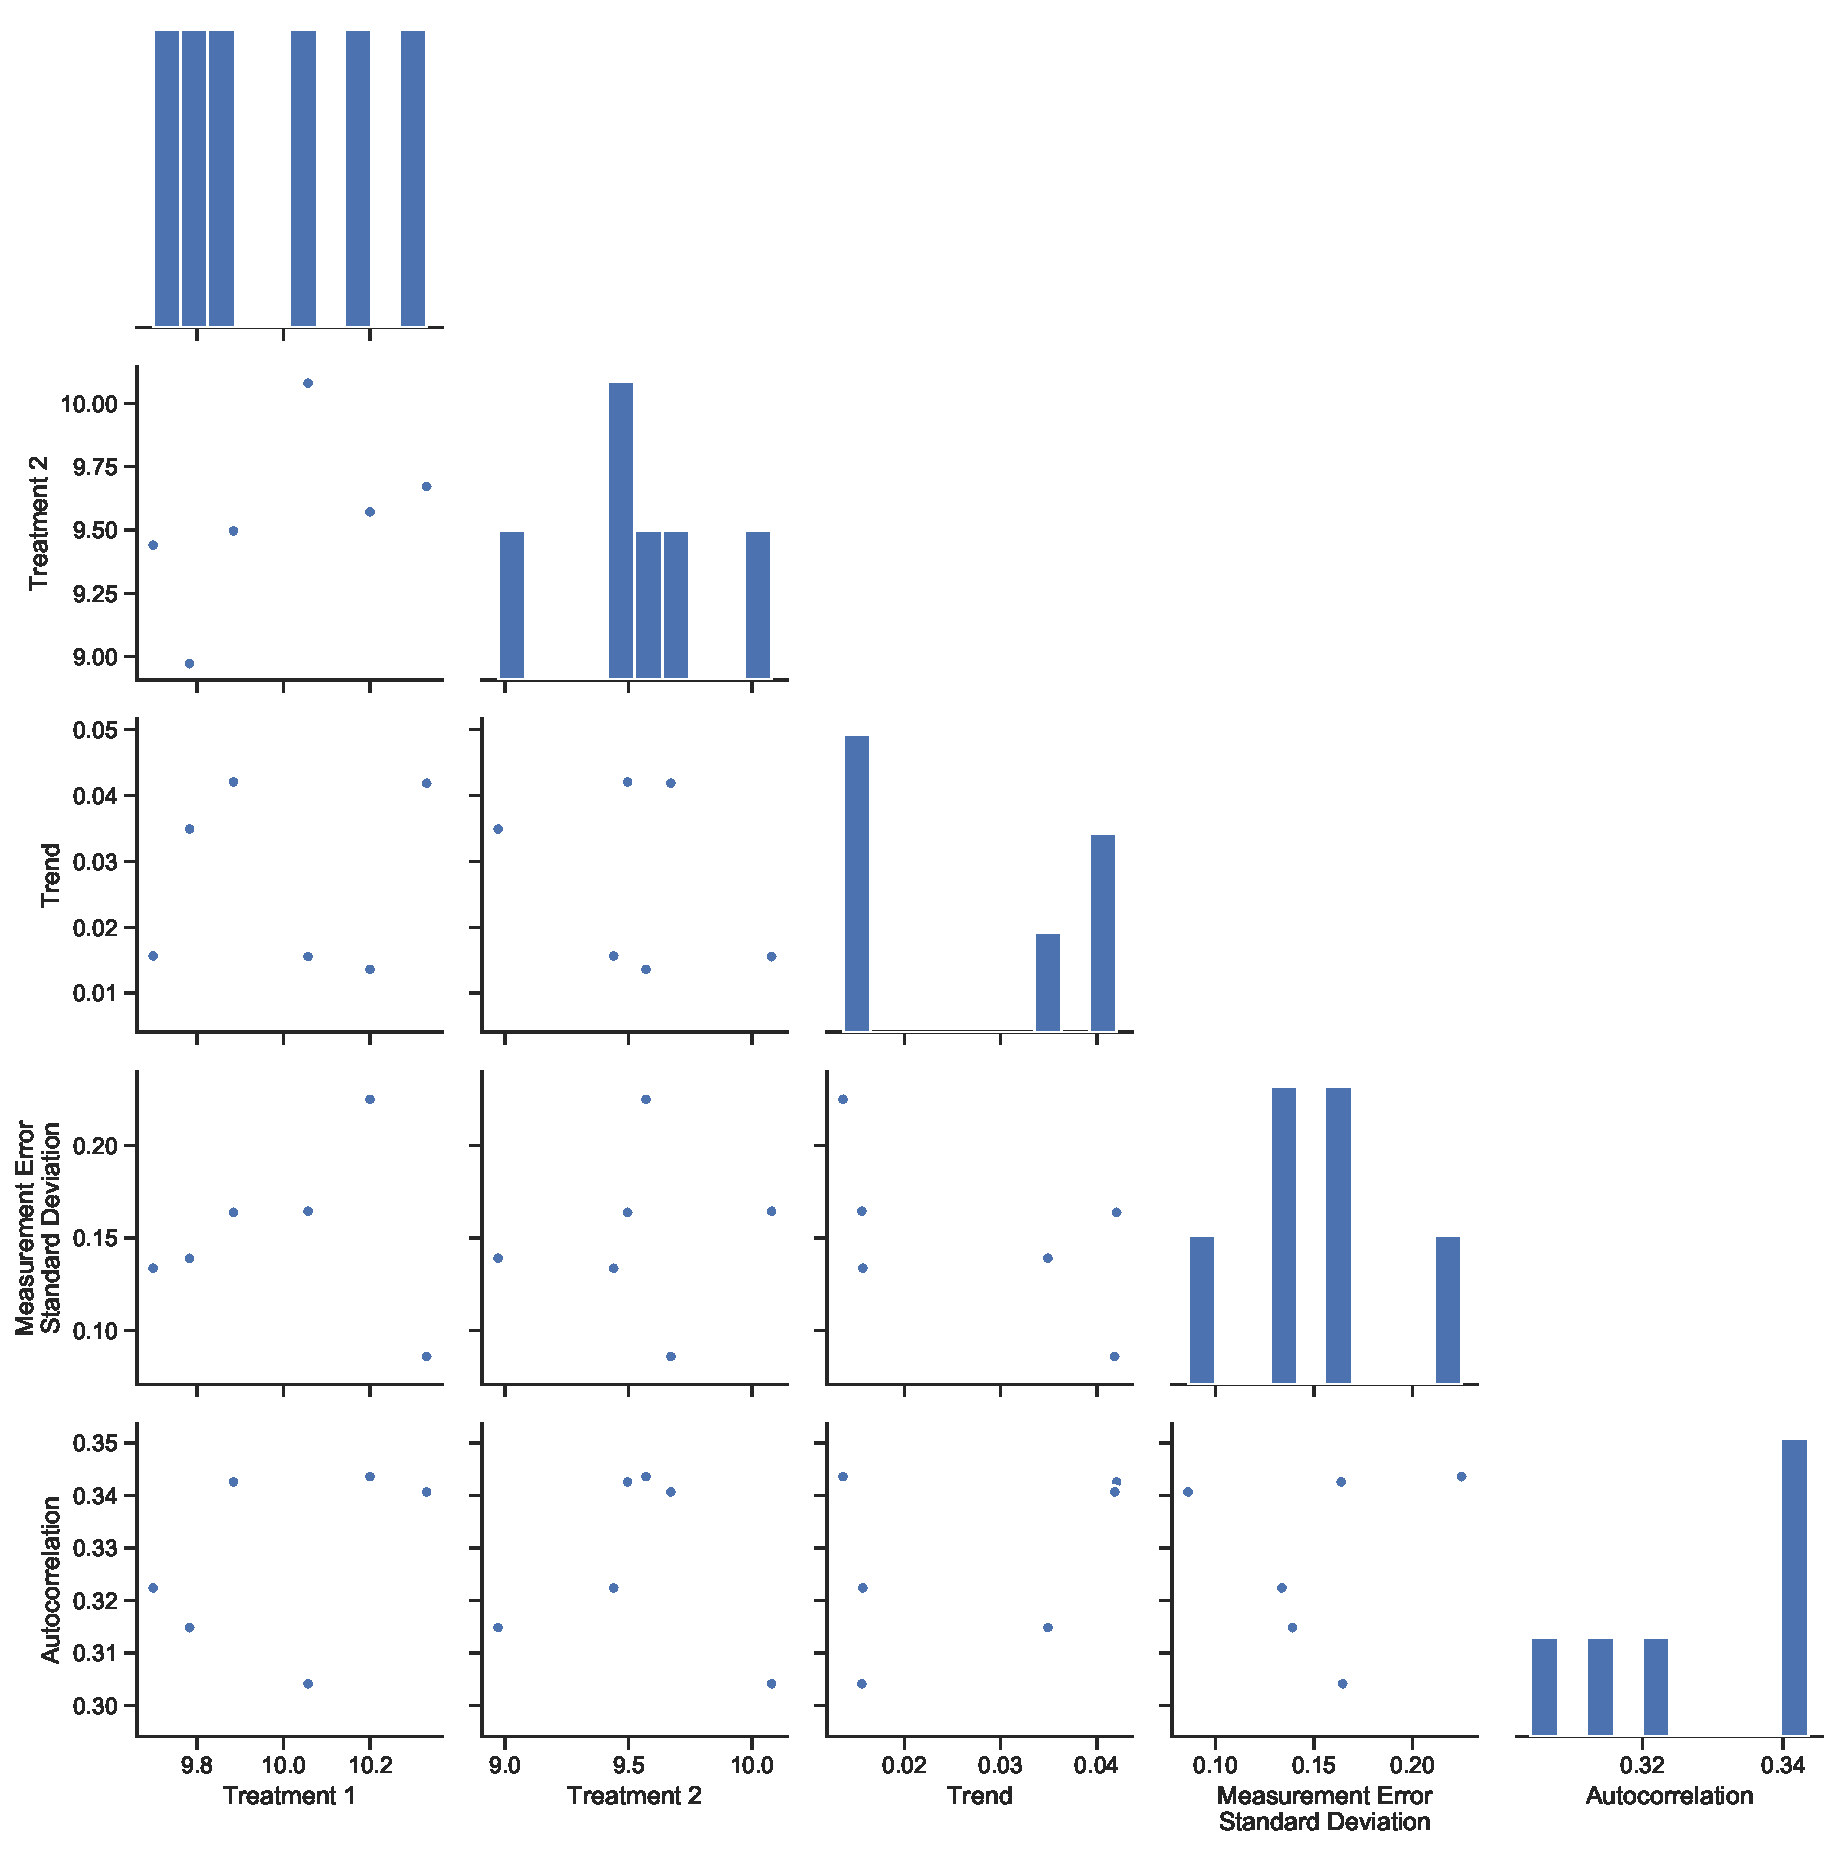
\includegraphics[width=\textwidth,height=\textheight,keepaspectratio]{patient_parameter_relationships.pdf}
    \par
}
\bigskip

\bigskip
{
    \centering
    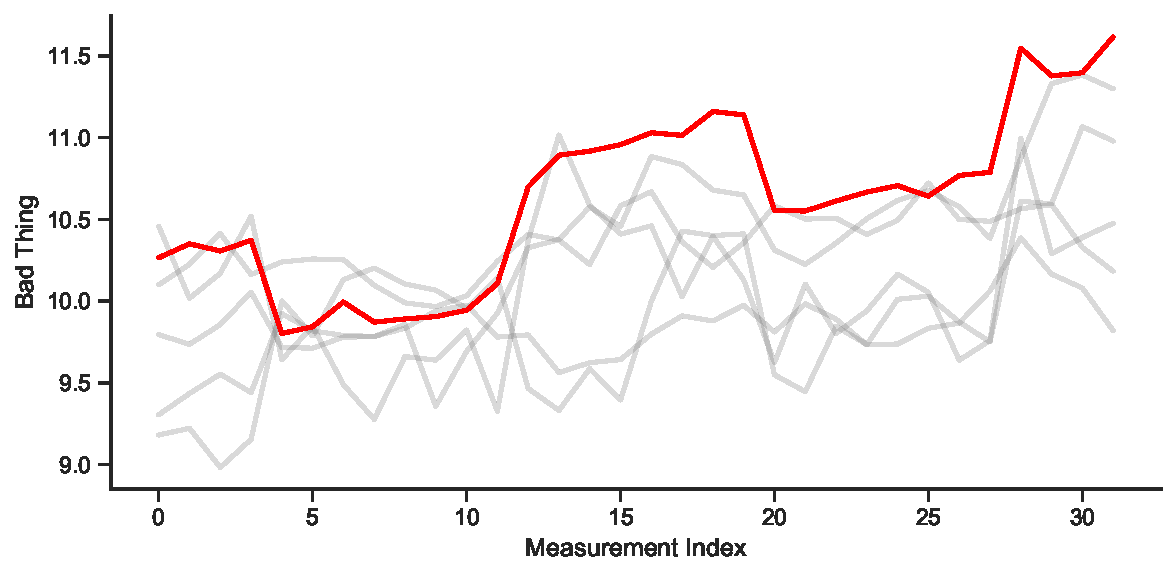
\includegraphics[width=\textwidth,height=\textheight,keepaspectratio]{measurements_timeline.pdf}
    \par
}
\bigskip



What makes the simulated data hierarchical?

picture of the hierarchical parameter structure used to create the data

\section{Analyzing a Single Trial}\label{1trial}

PYMC3 requires that we appropriate give it functional forms for likelihoods to
represent the information from the data. This can be bit tricky when it is clear
that likelihood does not take form a well known distribution. For these cases we
must define the log-likelihood function of the likelihood manually.

Theano is a package that allows us to define functions involving array
operations and linear algebra

\subsection{Defining the Model}\label{1model}

\begin{def}\label{simulationmodel}
    \begin{equation}\label{}
        y_t = \mu + Z_t\theta + \epsilon_t
    \end{equation}
\end{def}where \(\mu\) is the baseline \(\theta\) is the treatment effect with
\(Z_t\) being an indicator variable that is 1 when \(t\) is within a period
where treatment was applied and 0 otherwise and finally \(\epsilon_t \sim
N(0,\sigma^2) \) is the error term.

Priors:

\begin{def}\label{simulationmodel}
    \begin{equation}\label{}
        \mu \sim N(10, 3^2)
    \end{equation}
    \begin{equation}\label{}
        \theta \sim N(0, 1^2)
    \end{equation}
    \begin{equation}\label{}
        \epsilon \sim HalfCauchy(loc=0, scale=10)
    \end{equation}
\end{def}

Defining the priors and incorporating our previous knowledge.

Defining the model in a technical sense with STAN, with mention of the problems
that have to be considered

\subsection{Results}\label{1results}

\section{Analyzing Multiple Trials With Hierarchical Models}\label{pooling}

With the shape parameter we can initialise the parameters as vectors with the
length of out number of patients. This way each patient get her own parameter.

\subsection{Defining the Model}\label{hiermodel}

\begin{def}\label{simulationmodel}
    \begin{equation}\label{}
        y_t = \mu_i + Z_t\theta_i + \epsilon_i
    \end{equation}
\end{def}where \(\mu_i\) is the baseline of the patient \(i\), \(\theta_i\) is
the treatment effect with \(Z_t\) being an indicator variable that is 1 when
\(t\) is within a period where treatment was applied and 0 otherwise and finally
\(\epsilon_i \sim N(0,\sigma_i^2) \) is the error term.

Individual parameters relation to population distribution:

\begin{def}\label{simulationmodel}
    \begin{equation}\label{}
        \mu_i \sim N(\mu_{pop}, \sigma_{pop}^2)
    \end{equation}
    \begin{equation}\label{}
        \theta_i \sim N(\theta_{pop}, \sigma_{pop}^2)
    \end{equation}
    \begin{equation}\label{}
        \sigma_i \sim HalfCauchy(loc=0, scale=\sigma_{pop})
    \end{equation}
\end{def}

Defining priors for the population distribution:

\begin{def}\label{population_priors}
    \begin{equation}\label{}
        \mu_{pop} \sim N(10, 3^2)
    \end{equation}
    \begin{equation}\label{}
        \sigma_{pop} \sim HalfCauchy(loc=0, scale=10)
    \end{equation}
    \begin{equation}\label{}
        \theta_{pop} \sim N(0, 1^2)
    \end{equation}
    \begin{equation}\label{}
        \sigma_{pop} \sim HalfCauchy(loc=0, scale=10)
    \end{equation}
    \begin{equation}\label{}
        \sigma_{pop} \sim HalfCauchy(loc=0, scale=10)
    \end{equation}
\end{def}

\subsection{Results}\label{hierresults}

Visualization of the shrinkage

% \addcontentsline{toc}{chapter}{Bibliography}

\begin{thebibliography}{4}

    \bibitem{nofone}
    Richard L. Kravitz, Naihua Duan, Sunita Vohra, Jiang Li: Introduction to to
    N-of-1 Trials: Indications and Barriers in Design and Implementation of
    N-of-1 Trials: A User's Guide, AHRQ, 2014.

    \bibitem{costs}
    Wilson D. Pace, Elizabeth W. Staton, Eric B. Larson: Financing and Economics
    of Conducting N-of-1 Trials in Design and Implementation of N-of-1 Trials: A
    User's Guide, AHRQ, 2014.

    \bibitem{stat}
    Christopher H. Schmid, Naihua Duan: Statistical Design and Analytic
    Considerations in Design and Implementation of N-of-1 Trials: A User's
    Guide, AHRQ, 2014.

    \bibitem{clinbayes}
    Christoper J. Gill, Lora Savin, Christopher H. Schmid: Why clinicians are
    natural Bayesians, British Medical Journal 2005;330(7499):1080-1083.

    \bibitem{diseaseburden}
    Colin D. Mathers, Dejan Loncar: Projections of global mortality and burden
    of disease from 2002 to 2030, PLoS medicine 2016;3.11:e442.

    \bibitem{cgm}
    Irl B. Hirsch, et al.: Clinical application of emerging sensor technologies
    in diabetes management: consensus guidelines for continuous glucose
    monitoring (CGM). Diabetes Technology and Therapeutics 2018;10.4:232-246.

    \bibitem{kruschke}
    John K. Kruschke: Doing Bayesian Data Analysis: A Tutorial With R, JAGS, and Stan
    (2nd), Academic Press, 2014.

    \bibitem{gelman}
    Andrew Gelman, John B. Carlin, Hal Stern, David Dunson, Aki Vehtari, Donald B.
    Rubin: Bayesian Data Analysis, CRC Press, 2013

    \bibitem{HTE1}
    Peter Rothwell: External Validity of Randomised Controlled Trials: “To Whom Do the
    Results of This Trial Apply?”, Lancet, Jan 1-7 2005;365(9453):82-93.15

    \bibitem{HTE2}
    Peter Rothwell: Treating individuals 2. Subgroup Analysis in Randomised Controlled
    Trials: Importance, Indications, and Interpretation, Lancet, Jan 8-14
    2005;365(9454):176-186.16

    \bibitem{HTE3}
    Diane Warden, John Rush, Madhukar Trivedi, et al.: The STAR*D Project Results: A Comprehensive Review of Findings, Current Psychiatry Reports, Dec 2007;9(6):449-459

    \bibitem{HTE4}
    David Kent, Peter Rothwell, John Ioannidis, et al.: Assessing and Reporting Heterogeneity in
    Treatment Effects in Clinical Trials: A Proposal, Trials, 2010;11:85

\end{thebibliography}
\end{document}
